	The Stochastic version of the  Duffing Van Der Pol Oscillator 
	\begin{equation}\label{eqn:StochasticDvdPOscillator}
		\ddot{y}= (\alpha +\sigma_1 \dot{W}_1)y+
			\beta \dot{y} - y^3 +\sigma_2 \dot{W_2}
	\end{equation}
is a standard test case for the theory of stochastic bifurcation 
\cite{He2004, Arnold1998, Keller1999, Schenk-Hoppe1996a, Schenk-Hoppe1996b, Wei1997}. If one allows that both, 
$\alpha$, $\beta$ to be bifurcation parameters, then this model represents the generic normal form of the double zero 
co-dimension. In addition, there are many physical problems where its dynamics are described by the above SDE. For
example, mechanical systems as aircraft at high angles of attack, exhibit such co-dimension two instabilities. Also,
this SDE represents the motion of a thin panel under supersonic airflow \cite{dowell1966nonlinear}.
%
\begin{align}
	dX_t^{(1)}
		&= X_t^{(2)} dt \label{eqn:GenDuffingVanDerPolSDE1}\\
	dX_t^{(2)} &=
	\left\{
		\alpha X_t^{(1)} 
		- \left( X_t ^ {(1)} \right) ^ 3
		- \left( X_t ^ {(1)} \right) ^ 2 X_t ^ {(2)}
		+\beta X_t^{(2)}
	\right\}dt
	+ \sigma_1 X_t^{(1)} dW^{(1)}
	+ \sigma_2 dW^{(2)}
	\label{eqn:GenDuffingVanDerPolSDE2}
\end{align}
Note that we can rewrite the drift term as 
\begin{align*}
	dX^{(1)}_t &= dX^{(2)}_t\\
	dX^{(2)}_t &= 
		\left(
			\beta - \left(X^{(1)}_t \right)^2
		\right) X^{(2)}_t
		+ X^{(1)}_t
		\left(
			\alpha - \left(X^{(1)}_t \right)^2
		\right)
\end{align*}
So using the scheme \eqref{eqn:SteklovSchem2} we get the Steklov scheme
\begin{align*}
	X^{(1)}_{k+1} &= X^{(1)}_k + hX^{(2)}_k\\
	X^{(2)}_{k+1} &= 
		\exp \left(
			h a_2
		\right)
		\left(
			X^{(2)}_k + \frac{b_2}{a_2}
		\right)
		- \frac{b_2}{a_2}
		+\sigma_1 X_k^{(1)} \Delta W^{(1)}_k
		+\sigma_2 \Delta W^{(2)}_k
		\\
	a_2 &:= \beta-X^{(1)}_k X^{(1)}_{k+1}, \qquad 
	b_2 := 
		X^{(1)}_{k+1} \left(
			\alpha -X^{(1)}_{k}X^{(1)}_{k+1}
		\right)
\end{align*}
In \Cref{fig:DuffingVanDerPolSDE} we compare the performance of the Euler-Maruyama and SSLS schemes on a 
deterministic and multiplicative noisy setting.
%\pagebreak
%	\newgeometry{left=1.75cm, bottom=3cm}
\begin{figure}[htb]
	\subfloat[]{
		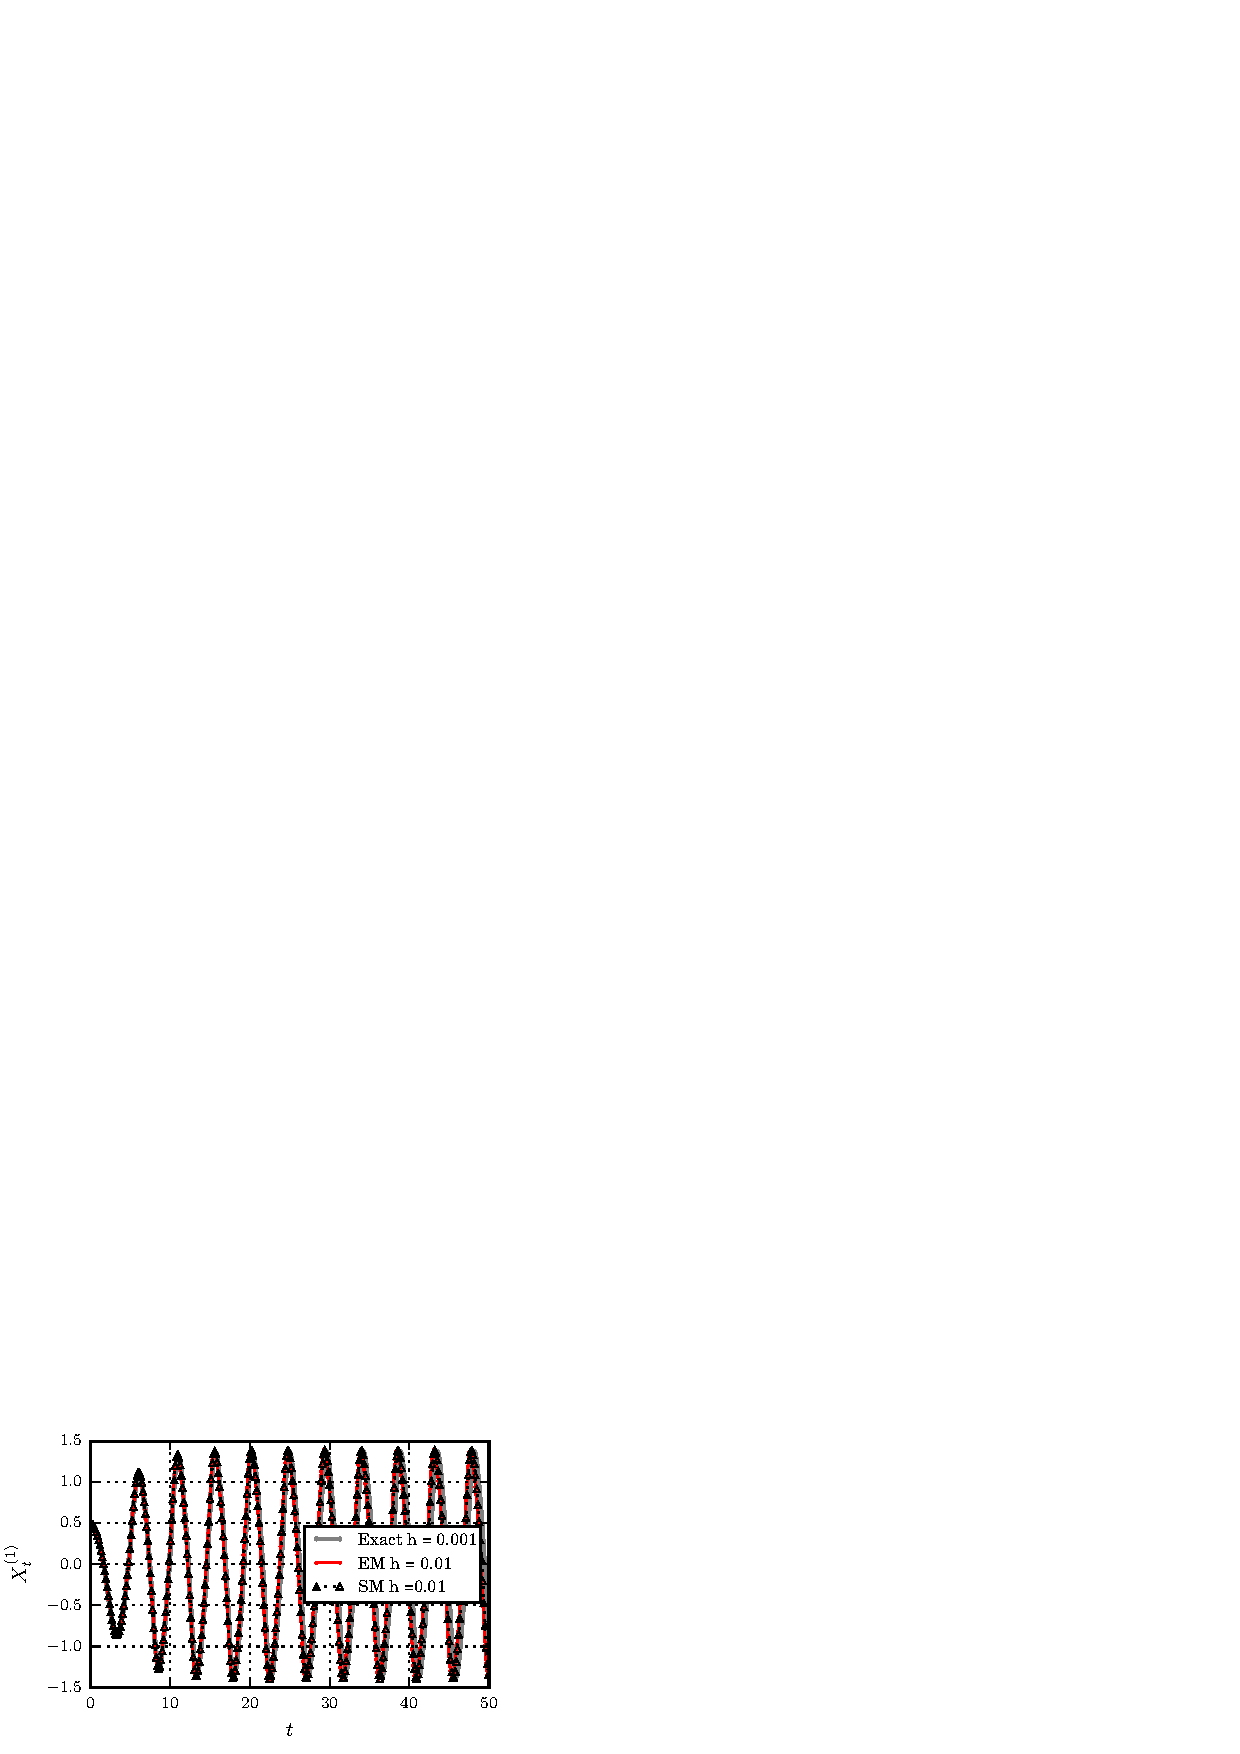
\includegraphics{./papers/paperB/figures/X1DuffingVanDerPolSchenke-2.png}
		\label{subfig:X1DuffingVanDerPolSchenk}
	}
	\subfloat[]{
		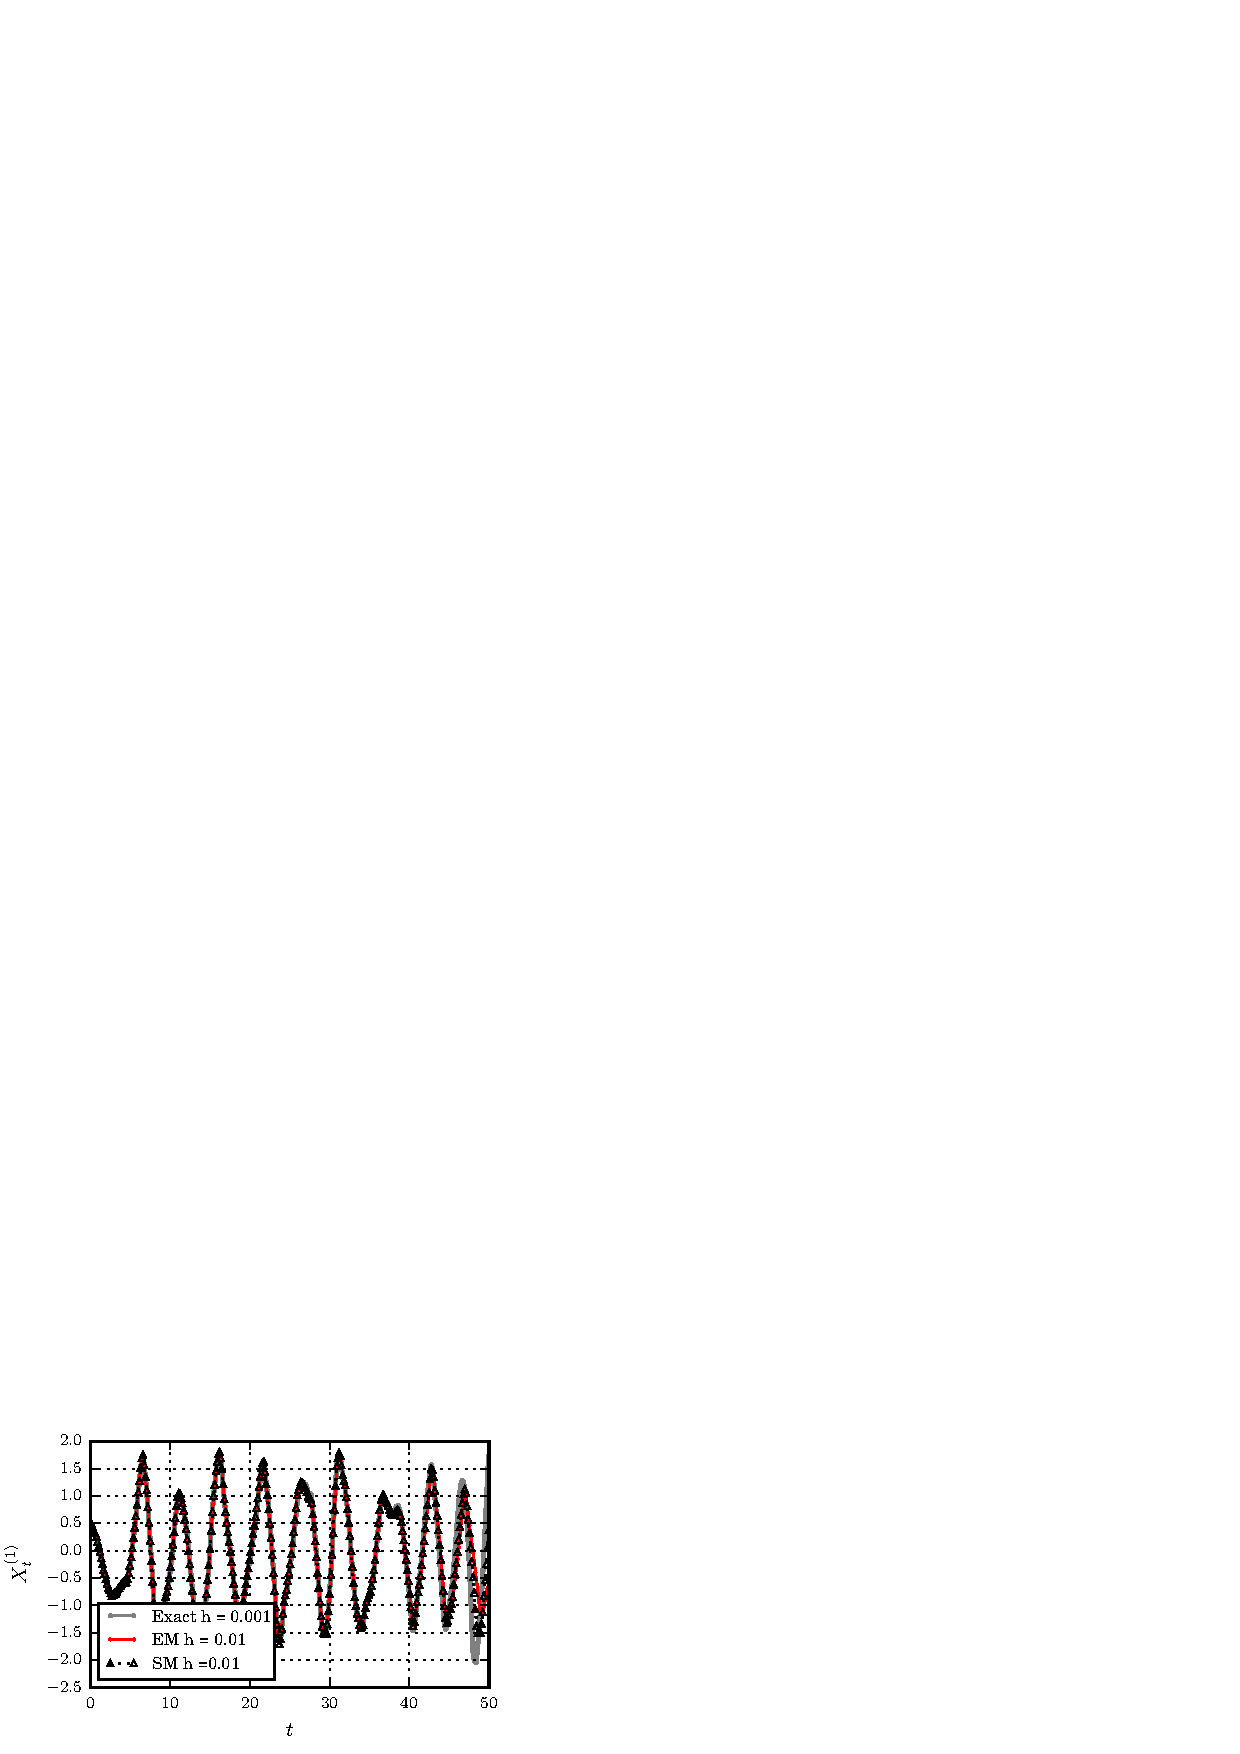
\includegraphics{./papers/paperB/figures/StoX1DuffingVanDerPolSchenke-2.png}
		\label{subfig:StoX1DuffingVanDerPolSchenk}
	}\\
	\subfloat[]{
		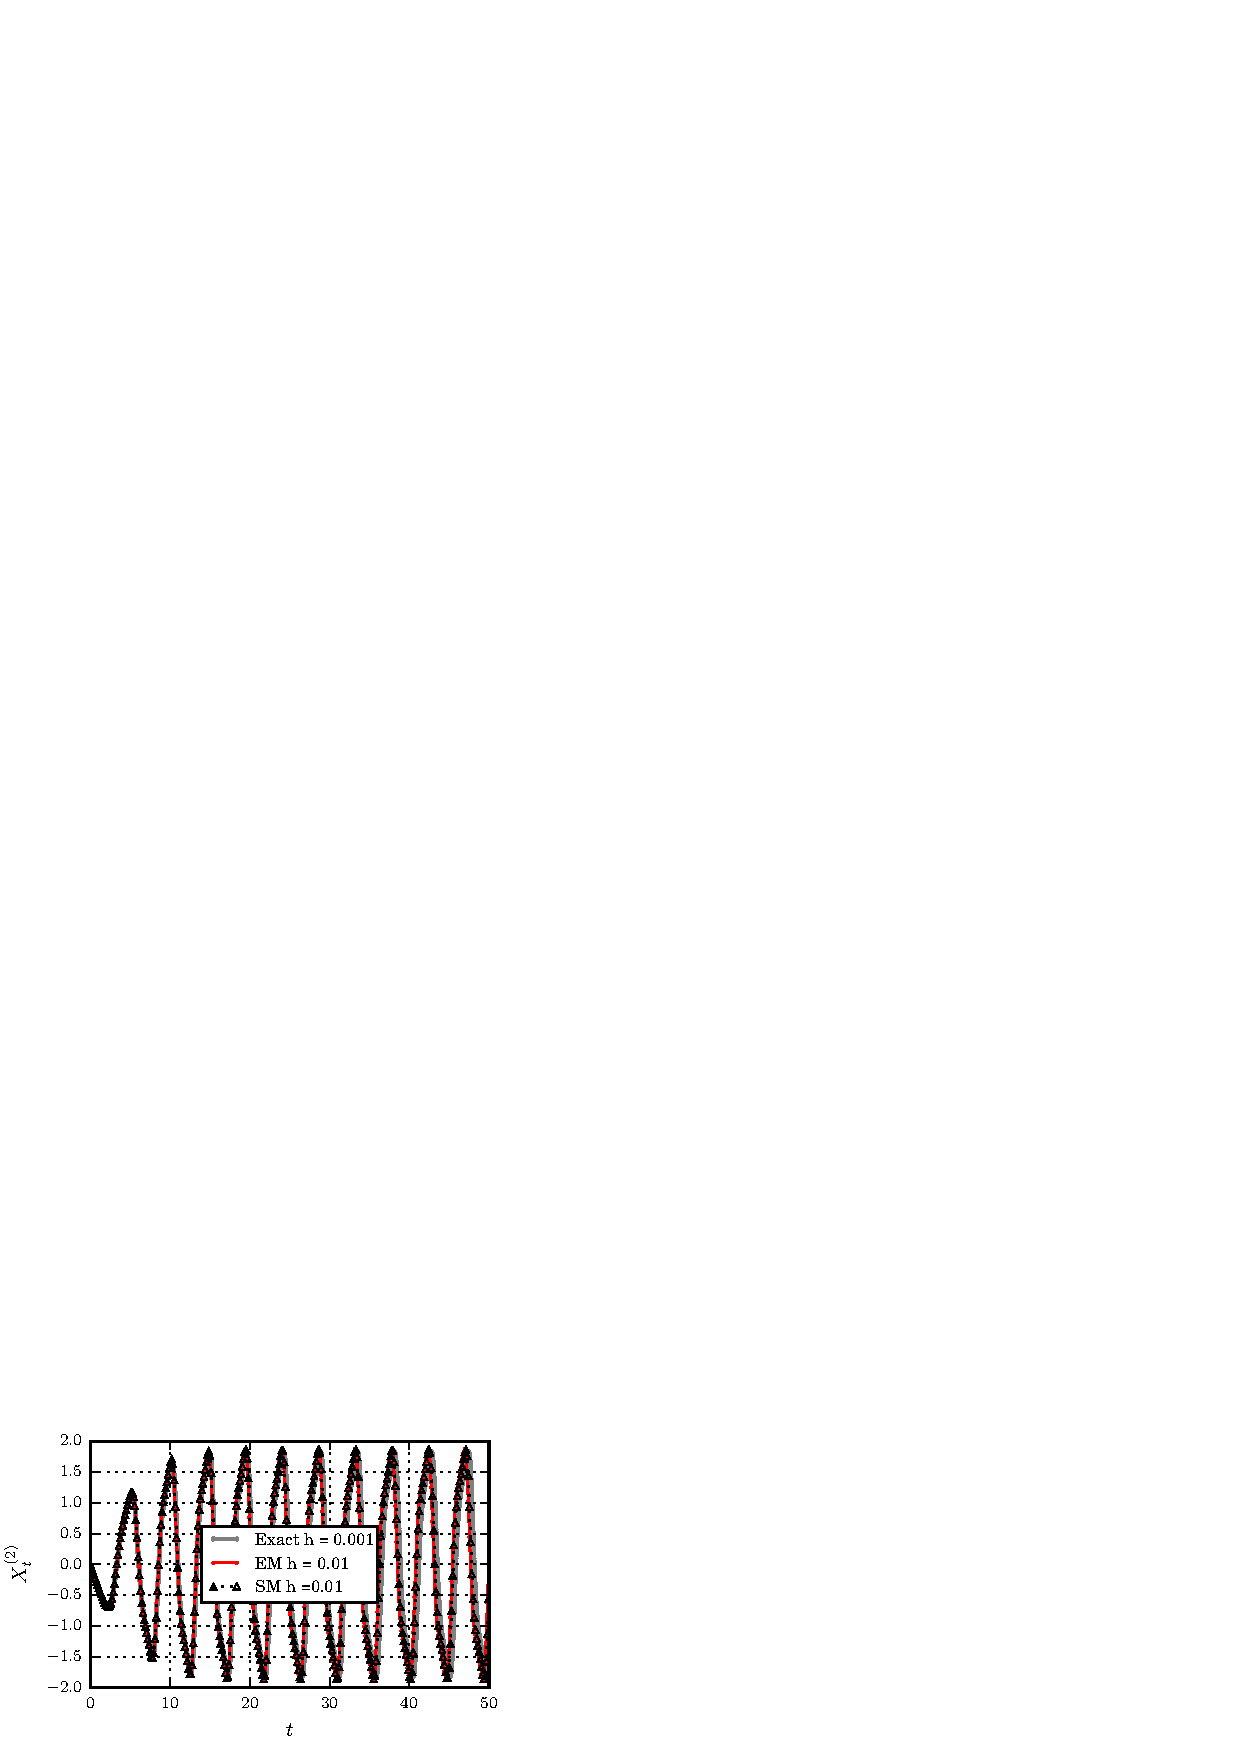
\includegraphics{./papers/paperB/figures/X2DuffingVanDerPolSchenke-2.png}
		\label{subfig:X2DuffingVanDerPolSchenke}
	}
	\subfloat[]{
		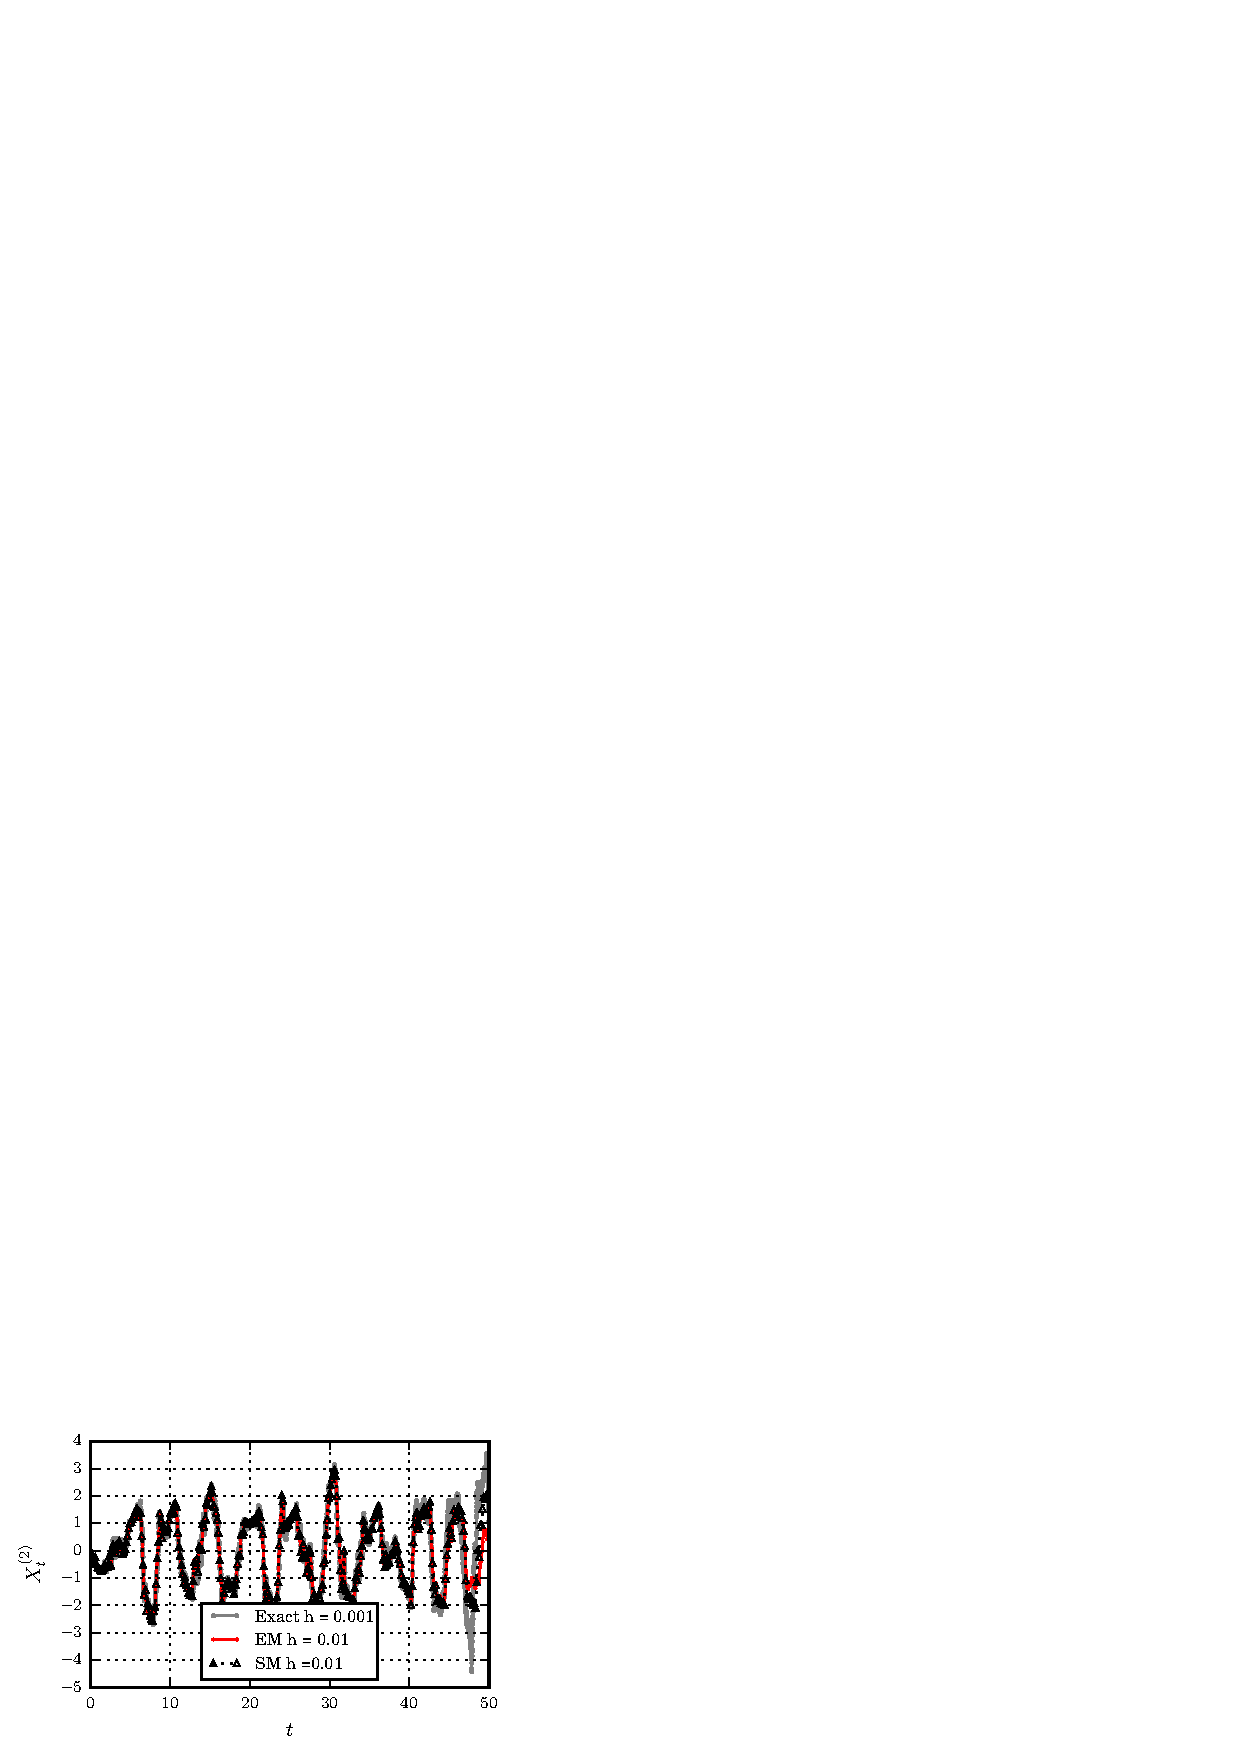
\includegraphics{./papers/paperB/figures/StoX2DuffingVanDerPolSchenke-2.png}
		\label{subfig:StoX2DuffingVanDerPolSchenk}
	}\\
	\subfloat[]{
		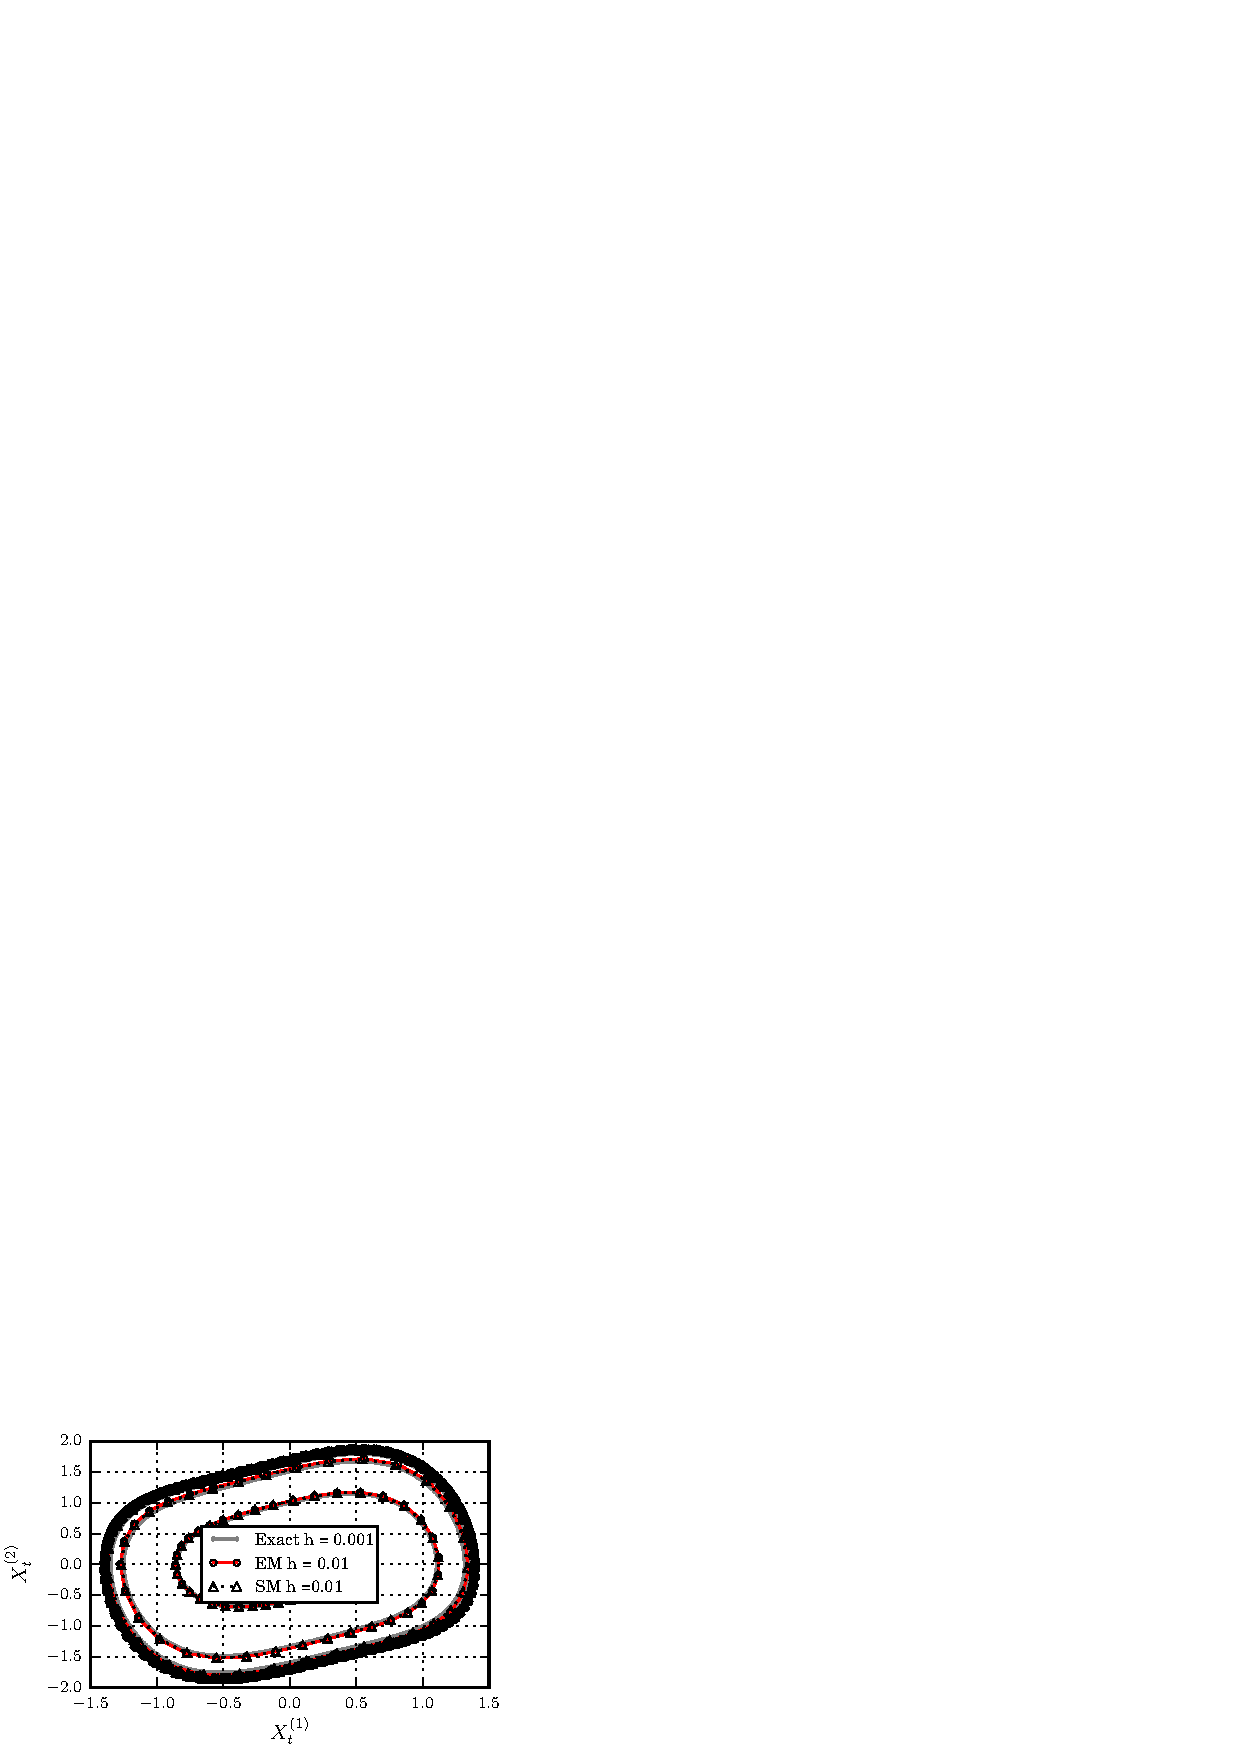
\includegraphics{./papers/paperB/figures/PhasePotraituffingVanDerPolSchenk.png}
		\label{subfig:PhasePotraituffingVanDerPolSchenk}
	}
	\subfloat[]{
		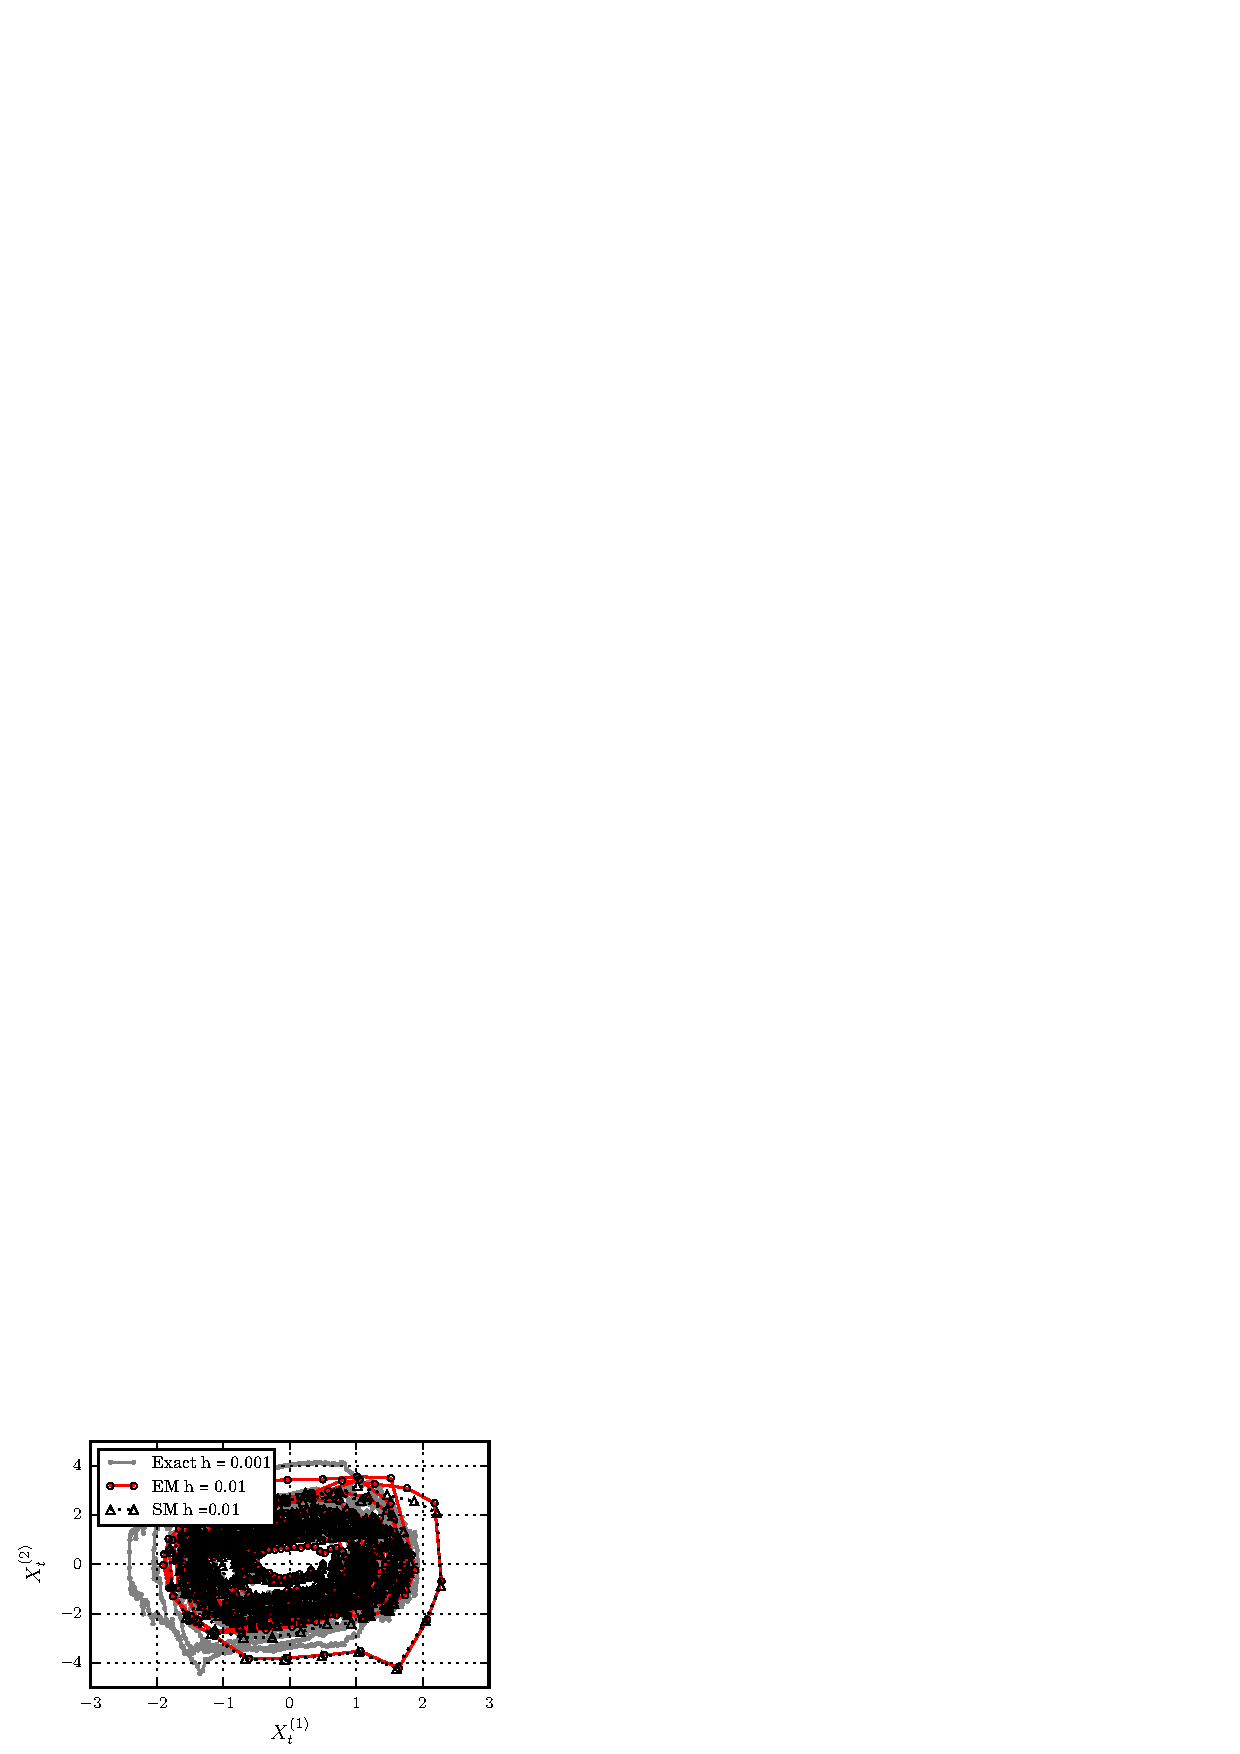
\includegraphics{./papers/paperB/figures/StoPhasePotraituffingVanDerPolSchenk.png}
		\label{subfig:StoPhasePotraituffingVanDerPolSchenk}
	}
	\caption{
		Simulation of the Duffing Van Der Pol noisy oscillator 
		\crefrange{eqn:GenDuffingVanDerPolSDE1}{eqn:GenDuffingVanDerPolSDE2} with the EM and SSLS schemes.
		The "Exact" gray line denotes a EM approximation with a step size of $h=\num{1e-3}$. The red and 
		black dashed lines represents the underlying  schemes with
		$h = \num{0.01}$,
		$T = \num{10000.0}$,
		$\alpha = -\num{0.5}$,
		$\beta = \num{0.5}$,
		$X=(\num{0.5}, \num{0})$,
		for the deterministic left graphs and with 
		$\sigma_1 = 1.0$,
		$\sigma_2 = 0.0$,
		multiplicative noise intensities.
	}
	\label{fig:DuffingVanDerPolSDE}
\end{figure}